\documentclass{article}

\usepackage[nodayofweek]{datetime}

\title{\textbf{Title} \\subtitle}
\author{Zhao Lyu}
%\date{2018-01-15}%change \today


\usepackage{amsmath, mathtools, amsfonts,amssymb,flexisym,enumitem,grffile,graphicx,tikz}
\usepackage{tkz-euclide}
%\usetikzlibrary{intersections,calc}
\usepackage{setspace}
\setlist[enumerate]{itemsep=0mm}
\graphicspath{{/home/user/Project199/Figures}}

\usepackage{amsthm}
\newtheorem*{definition*}{Definition}
\newtheorem{definition}{Definition}
\newtheorem{theorem}{Theorem}
\newtheorem*{theorem*}{Theorem}
\newtheorem*{lemma*}{Lemma}
\newtheorem{lemma}{Lemma}
\newtheorem*{claim*}{Claim}
\newtheorem{claim}{Claim}

\begin{document}

  \doublespacing %use setspace package
  \maketitle
  \singlespacing

  \newpage %separate title and contents
  \pagenumbering{gobble}
  \tableofcontents
  \newpage
  \pagenumbering{arabic}

  \section{Introduction}
  \newpage

  \section{Basic Definition}
    We first recall definitions of linear transformation and translation, and further introduce affine transformation, which we will use to prove stability of uniform mesh refinement and bisection in sections later. Then we introduce basic notions which we will use to present mesh refinement and show how they would work out.

    \subsection{Translation, Linear Transformation and Affine Transformation(pf for stability)}
      
      We define several classes of transformations that we use frequently.
      %sets\\
      linear, translation, affine transformation\\
      
      \begin{definition*}
        %$\textbf{Translation}$\\
         Let $\textbf{v}$ be a fixed vector, a $\textbf{Translation}$ ${T}_v$ on a figure applies as ${T}_v (\textbf{p}) = \textbf{p} + \textbf{v}$, for a vector $\textbf{p}$ in the figure which we translate.
      \end{definition*}
      A $\textit{translation}$ moves every point of a figure or space by the same distance in the same direction. A translation ${T}$ can be represented by an addition of a constant vector to every point.\\


      \begin{definition*}
      %\paragraph{Linear transformation}
      Let ${V}$ and ${W}$ be vector spaces over the same field $\textbf{K}$. We say a function $\mathit{f}: {V} \rightarrow {W}$ is $\textbf{linear transformation}$ if the following satisfied:\\
      \begin{align*}
      \mathit{f}(\textbf{u} + \textbf{v}) &= \mathit{f}(\textbf{u}) + \mathit{f}(\textbf{v}) \qquad \forall \textbf{u}, \textbf{v} \in{V},\\
      \mathit{f}(c\textbf{u}) &= c\mathit{f}(\textbf{u}), \qquad \forall \textbf{u} \in{V}, ~c\in\textbf{K}.
      \end{align*}
      \end{definition*}
      In other words, a linear transformation is a mapping between two vector spaces which preserves the operations of addition and scalar multiplication. Moreover, if ${V}$ and ${W}$ are finite dimentional, we can represent the linear transformation ${f}$ by a matrix ${M}$. For example, if ${M}$ is an ${m} \times {n}$ matrix, then ${f}$ is a linear transformation from $\mathbf{R}^n$ to $\mathbf{R}^m$. \\


      \begin{definition*}
      %\paragraph{Affine Transformation}
      An $\textbf{affine transformation}$ from $\mathbb{R}^n$ to $\mathbb{R}^n$ is of the form\\
      \begin{equation*}
      {F}(x) = {Ax} + {v}, \qquad {x}\in\mathbb{R}^n,
      \end{equation*}
      where ${A}$ is a linear transformation $\in\mathbb{R}^{n\times n}$, and  ${v}$ is a translation vector in $\mathbb{R}^n$\\
      \end{definition*}
      Affine transformation preserves points, lines and planes, but need not preserve point zero in a linear space in contrast to linear transformtion. So we see that translation and linear transformation is affine, but the opposite is not true.\\
      \indent
      The inverse mapping $F^{-1} = {x} \mapsto {A}^{-1}({x} - {v})$ is also an affine transformation. Clearly, we see that an affine transformation ${F}$ is invertible if and only if ${A}$ is invertible by the way we defined ${F}^{-1}$. Affine transformation helps carry results from one simplex to another simplex in our discussion, and more details are covered after introducing ${Simplices}$ and ${Triangulations}$ in the next section.

    \subsection{Simplices}
    simplices, subsimplices[DONE]\\
    affine set, affine transformation [DONE]
    how to affine transformation act on simplices [UPDATED]\\

    \noindent
    \begin{definition*}
    A $\textbf{k-simplex T}$ $\in{R}^n$ is a ${k-}$dimensional convex hull of ${k}$ + 1 vertices ${x}_0, \cdots, {x}_k \in \mathbb{R}^n$, which are affinely independent.\\
    \begin{equation*}
    \begin{split}
    {T} & = [{x}_0, \cdots, {x}_k ]\\
    & := \left\{{x} = \sum\limits_{i=0}^k \lambda_i {x}_i \Bigm| \sum\limits_{i=0}^k \lambda_i = 1 ~and~ 0 \leqslant \lambda_i \leqslant 1, 0 \leqslant i \leqslant k \right\}\\
    & := \left\{\lambda_0{x}_0 + \cdots + \lambda_k{x}_k \Bigm| \sum\limits_{i=0}^k \lambda_i = 1 ~and~ 0 \leqslant \lambda_i \leqslant 1, 0 \leqslant i \leqslant k \right\}.
    \end{split}
    \end{equation*}
    \end{definition*}
    If ${k} = n$, we can call ${k-simplex}$ without addressing the dimension. 2-simplices are also called ${triangle}$, and 3-simplices are called ${tetrahedra}$.

    \begin{definition*}
    %\paragraph{Subsimplices}
    An ${l-}$simplex ${S} = [{y}_0, \cdots, {y}_l]$ is called an $\textbf{l-subsimplex}$ of ${k-}$simplex ${T} = [{x}_0, \cdots, {x}_k]$, if indices $0 \leqslant {i}_0 \leqslant \cdots {i}_l \leqslant k$ with ${y}_i = {x}_i$, for $0 \leqslant l \leqslant k \leqslant n$.
    \end{definition*}
    Since there are $k+1$ vertices in ${k-}$simplex ${T}$, and $l+1$ vertices in ${l-}$subsimplex ${S}$, the number of ${l-}$subsimplex of ${k-}$simplex is $\binom{k+1}{l+1}$.


    %\paragraph{Simplices Equality}
    Consider simplices ${T} = [{x}_0, \cdots, {x}_k]$ and $\text{T\textprime} = [{y}_0, \cdots, {y}_k]$. We say these two simplices ${T}$ and ${T\textprime}$ are equal, i.e. ${T} = {T\textprime}$, if ${x}_i = {y}_i$ for $0 \leqslant i \leqslant k$. \\
    Note that the vertex ordering of simplex is fixed, so if two simplices ${T}$ and ${T\textprime}$ denote the same set but with different vertex ordering, they are not equal; instead, we say that ${T}$ coincides with ${T\textprime}$, i.e. ${T} \cong {T\textprime}$.

    \paragraph{Simplex under Affine Transformation}\mbox{}\\
    Instead of taking a sgingle variable $x\in\mathbb{R}^n$ for affine transformation, we can take a subset S $\subset \mathbb{R}^n$, which contains $x\in\mathbb{R}^n$. Then the transformed set $S\textprime$,
    \begin{equation*}
    S\textprime= {F}(x) = \left\{{F}(x) ~|~ x\in S \right\}.
    \end{equation*}
    Similarily, if we regard a k-dimensioanl simplex ${T} = {x_0, \cdots, x_k}$ as a subset $\in\mathbb{R}$, then the image of ${T}$ under affine transformation, denoted by $T\textprime$, is defined as below
    \begin{equation*}
    \begin{split}
    {T}\textprime & = {F}({T})\\
    & = \left\{{F}(x_0), \cdots , {F}(x_k)\right\}.
    \end{split}
    \end{equation*}
    We can see that ${T}\textprime$ is still a k-dimensional simplex. Furthermore, we can define ${F}({T}) = {AT} + {v}$, where $T$ is k-dimensional simplex $\in\mathbb{R}^n$. We might be curious about the relationship between simplices ${T}$ and ${T}\textprime$. Since vertices of a simplex are in a specific given order, so different vertex ordering leads to different simplices. Therefore, there exists an unique affine transformation such that ${T} = {T}\textprime$. Another important property of simplices is congruence.

    \begin{definition*}
    Two simplices T, T' are defined to be congruent if they can be obtained from each other by rotation, mirroring, scaling, and translation, i.e. if there exists a scaling factor c $\neq 0$, a translation vector $v\in\mathbb{R}^n$, and an orthogonal matrix $Q\in\mathbb{R}^{n\times n}$ such that
    \begin{equation*}
    T' \cong v + cQT
    \end{equation*}
    \end{definition*}
    \noindent
    When the two simplices $T, T'$ have same vertices but with different vertex ordering, we can translate it as $T' = F(T)$. Based on how we define the affine transformation, it's not hard to see that ${T} \cong {T}\textprime$. Then we say that ${T}$ and ${T}\textprime$ are in a same congruent class.



    \subsection{Shape Regularity Measure}\mbox{}\\
    $\textit{Shape measure}$ offers an objective mathematical measure on the overall quality of an Finite Element mesh, and this is helpful to explore the simplex regularity and to improve the quality of shapes of the elements. Different diffinitions are used for shape measure to present the quality of simplex, and we simply introduce the $\textit{geometric shape measure} ~\mu({T})$ of simplex ${T}$,  the one we use in this paper.

    \paragraph{Simplex Diameter and Volume}\mbox{}\\
    Let ${T} \in\mathbb{R}^n$ be a k-simplex where $k \leqslant n$, with vertices ${x}_0, \cdots, {x}_k \in\mathbb{R}^n$. We let diam$({T})^k$ denote the diameter of ${T}$, and we define
    \begin{equation*}
    %\operator???
    \operatorname{diam}({T})^k = \max \| x_i - x_j \|, \qquad 0\leqslant i\leqslant j\leqslant k.
    \end{equation*}
    In other words, diam$({T})^k$ is the longest distance between two vertices of ${T}$, which is equivalent to the length of the longest edge of ${T}$. If ${T}$ is a single vertex, then diam$({T}) = 0$.\\

    \noindent
    Let vol$^m$(${T}$) denote k-dimensional volume of ${T}$, and we have
    \begin{equation*}
    \operatorname{vol^k} ({T}) = \frac{1}{k!}\cdot|det(x_1-x_0, x_2-x_0,\cdots, x_k-x_0)|
    \end{equation*}
    \noindent
    If k = 0, then ${T}$ is a 0-dimensional simplex, i.e. a vertex. Then clearly, diam(${T}$) = 0, and vol$^0 ({T})$ = 1, the vol$^0$ of a single vertex is one.

    
    \paragraph{Shape Measure}\mbox{}\\
    Simplex diameter and volume are important to introduce shape measures. Here we define the {geometric shape measure} $\mu({{T}})$ of simplex ${T}$ by
    \begin{equation*}
    \mu({{T}}) = \frac{\operatorname{diam}({T})^k}{\operatorname{vol^k}({T})}, \quad\operatorname{vol^k(T) \neq 0}
    \end{equation*}
    If vol$^k(T)$ = 0, then we define $\mu({{T}}) = \infty$.\\
    To understand this definition, we can translate $\mu({{T}})$ as a measurement of how different the two variables, i.e. diam$({T})^k$ and vol$^k({T})$, are. For example, for a 3-dimensional simplex, i.e. a triangle, shape measure helps measure how narrow the triangle is. In other words, it measures how small the smallest angle of the triangle is. 

    \paragraph{Stability of a Simplex}\mbox{}\\
    The reason why we need shape measure is to help understanding whether a simplex $T$ is non-degenerate, and to quantify how degenerate or non-degenerate. Let $T$ be a k-dimensional simplex in $\mathbb{R}^n$. We say that a simplex $T$ is degenerate if and only if $\mu({T}) = \infty$, i.e. vol$_k(T) = 0$ approximating to 0.

    
    %???
    %\begin{tikzpicture}
    %\path (1,1) coordinate (A) (2.5, 2.5) coordinate (B) (3, 1) coordinate (C)
    %\draw (A) -- (B) -- (C) -- cycle
    %\end{tikzpicture}

    Observing two pictures above, we actually want the interior angles of the simple $T$, i.e. traingles in this example, to be uniformly bounded from zero. Thus vol$_2(T)$ will never go to 0.
    While cutting a simplex into smaller pieces, we want to keep those pieces uniformly bounded and avoid degenrate simplices. \\

    [ADDED LEMMA1: Congruent T1 T2 have same shape measure - ADDED]
    [Q1. CHECK]
    \begin{lemma*}
    If $T, T'$ are simplices that are congruent to each other, then $\mu(T) = \mu(T')$.
    \end{lemma*}
    \begin{proof}\mbox{}\\
    Since $T$ is congruent to $T'$, by definition, we have $T' \cong v + cQT$, where $c$ is scaling factor, $v$ is a translation vector and $Q$ is an orthogonal matrix. In fact, we will show that scaling, translation, roation or mirroring does not influence the shape measure of a simplex. \\
    To be specific, when sacling a simplex $T$ by a non zero factor $c$ to obtain $T'$, we have \(vol^k(T') = \displaystyle \frac{1}{k!}\cdot|det(cx_1-cx_0, cx_2-cx_0,\cdots, cx_k-cx_0)| = \frac{c}{k!}\cdot|det(x_1-x_0, x_2-x_0,\cdots, x_k-x_0)| = c\cdot vol^k(T)\). Since it scales over all vertices, $diam(T')^k = c\cdot diam(T)^k$. Therefore, we see $\mu(T') = \frac{diam(T')^k}{vol^k(T')} = \frac{c\cdot diam(T)^k}{c\cdot vol^k(T)} = \frac{diam(T)^k}{vol^k(T)} = \mu(T)$\\
    Moreover, translation over simplex $T$ by a nonsingular vector $v$ to obatin $T'$ will not influence the shape measure as well. Under translation, the ordering of vertices may be changed. However, by definition of simplex diameter and volume, difference in vertex ordering will not affect the absolute value of the determinant nor the longest distance between two vertices. Thus, we obtain that $\mu(T) = \frac{diam(T)^k}{vol^k(T)} = \frac{diam(T')^k}{vol^k(T')} = \mu(T')$.\\
    Similarily, roations and mirroring represented by an orthoginal matrix $Q$ will change the ordering of vertices, but again, simplex volume and diameter are independent of vertex ordering. Thus, we still obtain that $\mu(T)=\mu(T')$.\\
    Now we see the shape measure is independent of scaling, translation, rotation or mirroring. Thus a simplex $T'$ which is obtained by these motions shares a same shape measure with $T$.
    
    [ORIGINAL: ]
    First, we show that volumes of k-simplices $T$ and $T'$ are the same, i.e. vol$^k (T)$ = vol$^k (T')$. By definition of congruence, we can see one difference between equality and congruence of two simplices is that congruence is independent of vertex ordering. Recall the definition of simplex volume. \(vol^k(T) = \displaystyle \frac{1}{k!}\cdot|det(x_1-x_0, x_2-x_0,\cdots, x_k-x_0)|\). Clearly, permutation of vertex $x_i$, where $0 \leq i \leq k$, will not influence the absolute value of the determinant. Both dividing by k!, we have vol$^k (T)$ = vol$^k (T')$.\\
    Moreover, by definition of congruence above, we can obatin $T'$ by applying rotation, mirroring, scaling, and translation over $T$. Thus, diam$(T')^k$, the longest distance between two vertices of $T'$, is equal to the longest distance between two vertices of $T$, diam$(T)^k$. Therefore, we have $\mu(T) = \frac{diam(T)^k}{vol^k(T)} = \frac{diam(T')^k}{vol^k(T')} = \mu(T')$.
    \end{proof}
    
    \subsection{Simplicial Complex(OR Triangulation)}
    \begin{definition*}
    A $\textbf{simplicial complex} ~~\mathcal T$ in $\mathbb{R}^n$ is a finite set of simplices in $\mathbb{R}^n$ that satisfies the following:
    \begin{enumerate}[label =\arabic*.]
      \item Any face of a simplex from $\mathcal{T}$ is also in $\mathcal{T}$.
      \item The intersection of any two simplices ${T}_1, {T}_2 \in \mathcal{T}$ is a face of both ${T}_1$ and  ${T}_2$.
    \end{enumerate}
    \begin{figure}[b]
    \centering
    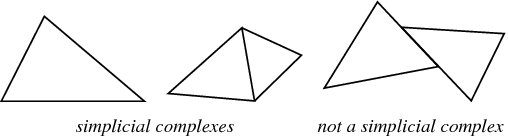
\includegraphics[width=60mm]{Figures/SimplicialComplex.png}
    \caption{Simplicial Complex Example and Counterexample}
    \end{figure}
    \end{definition*}
    In other words, the first condition asks $\mathcal{T}$ to be closed under subsimplices, and the second condition asks that the intersection of any two simplices is either a common subsimplex or empty because the empty set is a face of every simplex. Examples in 2D are shown in Figure.1. \\
    \indent
    Any subset ${T\textprime}\in{T}$ that is itself a simplicial complex is called a $\textit{subcomplex}$ of ${T}$. A $\textit{simplicial k-complex} ~~\mathcal T$ is a simplicial complex where the largest dimension of any simplex in $\mathcal T$ is ${k}$. So a simplicial 2-complex must not contain tetrahedra or higher dimension simplices. The 0-complex of ${T}$ is called a $\textit{vertex set}$ of ${T}$. We can also think simplicial complex as a space with a triangulation, which is the division of a surface or a plane polygon into a set of 2-simplices. The constrains of triangulation will be discussed in ? section.\\

    \paragraph{Simplicial Complex under Affine Transformation}\mbox{}\\
    Extending further from simplex under affine transformation, now we know that simplicial complex is just a finite set of simplices. Therefore, we can define the Transformed Simplicial Complex $F(\mathcal{T})$ as follows
    \begin{equation*}
    F(\mathcal{T}) := \{F(T) \quad \vert \quad T\in \mathcal{T}\}
    \end{equation*}
    If $\mathcal{T}$ is consistent, then $F(\mathcal{T})$ is also consistent by inheriting this property from $\mathcal{T}$.

    \paragraph{Shape Measure of Simplicial Complex}[DELETE???]\mbox{}\\
    We define shape measure of a simplex \(T \in\mathbb{R}^n$ as $\mu({{T}}) = \displaystyle \frac{\operatorname{diam}({T})^k}{\operatorname{vol^k}({T})}\). Now consider a simplicial complex $\mathcal{T}\in\mathbb{R}^n$, we define the geometric shape measure $\mu(\mathcal{T})$ as follows,
    \begin{equation*}
    \mu(\mathcal{T}) = \max_{T \in \mathcal{T}} \mu(T)
    \end{equation*}
    By definition, we see that the shape measure of a simplicial complex $\mathcal{T}$ is the supreme of the set of shape measures of all simplex $T\in\mathcal{T}$. If the largest shape measure of a simplex in this simplicial complex is bounded, then none of simplices in $\mathcal{T}$ is degenerate. In other words, if simplex $T_0 \in\mathcal{T}$ is non-degenrate, then simplicial complex $\mathcal{T}$ non-degenerate.
    [Correct?? Pf needed???]


    \section{Refinement Strategy in General}
    Refinement is a procedure of mesh modification in which we can divide a regular domain into smaller pieces under boundary constrains. This process can be applied recursively to simplify some differential equations by generating smaller pieces of the domain. Let us first introduce triangulation to help undertsand refinement on a simplex. Generally speaking, we can think triangulation as a subdivision of a plane into triangles. Definition below is a more formal way to take when extending to higher dimension.
    \begin{definition*}
    A triangulation of $\mathbb R^n$ is subdivision into n-dimensional simplices such that intersection of any two simplices is either empty or sharing a common face, and any face of a simplex is in the triangulation.
    \end{definition*}
    Indeed, we say that this triangulation is consistent as it is not simply subdividing of a space. Moreover, the triangulation defined here can be treated equavalently as simplicial complex as it is a finite set of simplices satisfying\\
    1. Any face of a simplex from a triangulation is also in the triangulation,\\
    2. The intersection of any two simplices ${T}_1, {T}_2 $ in a triangulation is a face of both ${T}_1$ and  ${T}_2$ or empty.
    (Denote triangulation same as simplical complex $\mathcal{T}$)\\
    

    We can think a refinement of a simplex $T$ as a triangulation $\mathcal{T}$ which consists of smaller pieces of simplices of same type of the simplex $T$. Now consider a refinement of a simplicial complex. Let $\mathcal{T}$ and $\mathcal{T'}$ be two different simplicial complex covering a same domain $\Omega$. This means that the domain \(\Omega = \displaystyle \bigcup({T \vert T\in \mathcal{T}}) = \bigcup({T' \vert T\in \mathcal{T'}})\). We say that $\mathcal{T'}$ is a refinement of $\mathcal{T}$ if each simplex $T\in\mathcal{T}$ is in $\mathcal{T'}$ or the triangulation of $T$ is in $\mathcal{T'}$.

    As mentioned before, we may recursively apply a refinement strategy to help simplify some problems. By recursively taking refinment process from $\mathcal{T}_0$, we have a hierarchy triangulation $\mathcal{T}_k, k\in\mathbb{N}$, where $\mathcal{T}_k$ is a refinement of $\mathcal{T}_{k-1}$. 
    \begin{definition*}
    Let $\mathcal{T}_0$ be the initial simplicial complex in $\mathbb{R}^n$ where it starts from, then we define the hierarchy triangulation $\mathcal{T}_k$ as follows
    \begin{equation*}
    \mathcal{T}_k := \bigcup\{refinement~of~simplex~T ~\vert ~T\in\mathcal{T}_{k-1}\}, \quad k\in\mathbb{N}
    \end{equation*}
    \end{definition*}

    \subsection{Stability of Refinement}
    \begin{definition*}
    We say a refinement strategy is $\textbf{stable}$ if there exists a constant C $>$ 0 such that $\mu(T)<$ C for all simplices $T$.
    \end{definition*}
    
    \begin{theorem*}
    If the number of congruence classes, obtained by applying the refinement of a non degenerate simplex $T$ initially, is finite, then the refinement strategy is stable.[UPDATED]
    \end{theorem*}
    \begin{proof}
    Idea:\\
    1. $T_0$ is non-degenrate, then $\mathcal{T_0}$ is non-degenerate.\\
    \begin{claim*}
    Refinement strategy over initial simplicial complex $\mathcal{T_0}$ produces only non-degenerate simplicies $T$.
    \begin{proof}
    We prove this claim by induction.
    Clearly, the base case is true since it is given that all simplices $T$ in $\mathcal{T}$ are non-degenerate. For induction, suppose simplices in simplicial complex $\mathcal{T}_k$ is non-degenerate, i.e. given C $> 0, \mu(T) < C, ~\forall T \in\mathcal{T}_k$. Apply te refinement strategy on $\mathcal{T}_k$, and then we obtain $\mathcal{T}_{k+1} = \bigcup\{refinement~of~simplex~T ~\vert ~T\in\mathcal{T}_{k}\}, \quad k\in\mathbb{N}$. [connection???: f simplex $T_0 \in\mathcal{T}$ is non-degenrate, then simplicial complex $\mathcal{T}$ non-degenerate.]
    \end{proof}
    \end{claim*}

    \begin{claim*}
    If the number of congruence classes is finite, then the number of shape measure is finite, and there exist a common bound C $> 0$ such that C $\geq \mu(\mathcal{T})$.
    \begin{proof}
    We proved that simplices in same congruence classes share the same shape measure. If we have finite number of congruence classes, clearly we have finite number of shape measure. When all simplices are non degenerate, we always have an upper bound for their shape measure $\mu(T)$. With the finite number of shape measure, we may set C as the maximum of all upper bounds of shape measures. And therefore C $\geq \mu(\mathcal{T})$
    \end{proof}
    \end{claim*}

    Since $T_0$ is non-degenrate, then $\mathcal{T_0}$ is non-degenerate. Moreover, we know there exists a common bound C for all shape measures since the number of congruence classes is finite. Therefore, we proved the stability.[UPDATED]
    \end{proof}

    
    2. Finite number of congruence classes, then finite number of bounds?\\
    3. Summary: each $\mathcal{T}$ is non-degerante + finite number of $\mathcal{T}$ = all $\mathcal{T}$ is non-degenrate. By def, the refinement strategy is stable.

    [Q2. NEED CORRECTION]
    
    \subsection{Consistency of Refinement}

    \section{Uniform Refinement}
    [Al of uniform refinement in 2-d, show it's stable and consistent]
    \subsection{2D -[UPDATED]}
    One popular refinement strategy is $red/green$ refinement proposed by R. E. Bank et al. The red refinement here is regular refinement which divides a triangle into four congruent smaller triangles by connecting midpoints of its three edges. The green refinement is irregular refinement which connects the refined edge midpoint to its opposite corner.[PIC-NEED TO BE UPDATE]\\

    Let $T = [x^0, x^1, x^2]$ be the triangle to be refined, and denote $x^{ij}$ as the midpoint of the edge between $x^i$ and $x^j$.\\
    \textbf{Algorithm} Red refinement in 2D \{\\
    $T_1 := [x^0, x^{01}, x^{02}]; \qquad T_2 := [x^{01}, x^{1}, x^{12}];$\\
    $T_3 := [x^{02}, x^{12}, x^2]; \qquad T_4 := [x^{01}, x^{12}, x^{02}];$\\
    \}
    Subdividing a triangle by connecting its midpoint, we obtain four congruent simplices $T_1, T_2, T_3$ and $T_4$. The green refinement is applied on one refined edge on which we may confront with degenerate simplices. We will never touch and refine such simplices to avoid them from degenerating.

    
    Clearly, the red refinement strategy is stable since it produces a finite number of triangles congruenct to the original simplex. Meanwhile, we preserve consistency by bisecting triangles with one refined edge and never refine them any further. Therefore, we obtain stability and consistency through red and green refinement.

    \subsection{3D}

    \section{Bisection}

    \newpage
    $\textbf{FIGHTING!!! ALMOST THERE WOOOOOOOT WOOOOOOOOOT}  \diagdown{(\bullet{ > }\omega{ < }\bullet{})} \diagup{}$


    [Bibliography - ADD]
    [CORRRECT TEXTIT for T, F T']
    -Simplicial complex is alwlays consistent by definition as touch edge is always a subsimplex...
    x-finite number of consistency class-->finite number of shape measure-->shape measure is bounded
    lemma: simplex in one consistency class has same shape measure(pf)
    \newpage
    Prev Q:\\
    1.\\
    Lemma 1 [UPDATED]\\
    Shape measure of simplicial complex [UPDATED]\\
    2. \\
    Simplex T degenerate [UPDATED]\\
    Shape measure of simplical complex  [UPDATED]\\
    3. \\
    thm pf: finite number of congruence classes leads to stable refinement strategy [UPDATED]\\
    4. \\
    uniform refinement 2D[UPDATED]

    Q:\\
    1. More for Uniform refinement 2d? code?\\
    2.
    bisection: newest vertex? longest?
   

    [Lemma 1: If $T_0$ and $T_1$ in a same congruence class, then the shape measure of these two simplices are the same] Iff??
    [If T0 is non degenerate, then simplicial complex is non degenerate]
    [Thm]A refinemetn strategy is stable if and only if the number of congruence classes, obtained by applying the refinement of a non generate simplex $T$ initially, is finite. [DELETED]
    [Al of uniform refinement in 2-d, show it's stable and consistent]

    note: distinguish refinement and uniform refinement? regular, global = uniform, local = bisection?


\newpage
\begin{thebibliography}{9}
\bibitem{MathWorld}
Weisstein, Eric W. "Simplicial Complex."
\\\texttt{http://mathworld.wolfram.com/SimplicialComplex.html}

\end{thebibliography}

  %\subsection{}
\end{document}